\documentclass[a4paper,12pt]{report}
\usepackage{amssymb}

\usepackage{ucs}
\usepackage[utf8x]{inputenc} % Input encoding for Greek characters
\usepackage[greek,english]{babel} % Language support

\newcommand{\en}{\selectlanguage{english}}
\newcommand{\gr}{\selectlanguage{greek}}

% \usepackage{algorithm2e}
% \usepackage{algorithm}
% \usepackage{algorithmic}
\usepackage{enumitem}
\usepackage{tcolorbox}
\tcbuselibrary{listingsutf8}
\usepackage{float}
\usepackage{amsmath}
\usepackage{graphicx} % For including images
\usepackage{titlesec} % Custom title formatting
\usepackage{fancyhdr} % For custom headers and footers
\usepackage{geometry} % For adjusting page margins

% Adjust the page margins to make content wider
\geometry{top=2.5cm, bottom=2.5cm, left=2.5cm, right=2.5cm}

% Redefine chapter formatting to make it smaller
\titleformat{\chapter}[display]
    {\normalfont\LARGE\bfseries} % Smaller size and bold for chapter heading
    {\chaptername\ \thechapter} % Chapter number format
    {15pt} % Space between chapter number and title
    {\bfseries} % Smaller size and bold for chapter title
\begin{document}

\begin{titlepage}
    \centering
    \vspace*{-3cm}
    % University logo
    \includegraphics[width=1\textwidth]{auth_logo.png} % Replace with your actual logo file

    % University name in Greek
    \textbf{\gr ΑΡΙΣΤΟΤΕΛΕΙΟ ΠΑΝΕΠΙΣΤΗΜΙΟ ΘΕΣΣΑΛΟΝΙΚΗΣ}
    \vspace{2cm}

    % Document title and subtitle in Greek
    \LARGE\textbf{\gr Ψηφιακή Επεξεργασία Εικόνας Αναφορά} \\
    \Large\normalfont{\gr Εργασία 3} \\
    \vspace{4cm}

    \gr
    \large
    \textbf{Διακολουκάς Δημήτριος} \\
    \textbf{AEM 10642}
    \vspace{2.5cm}

    \en
    \textit{Email: ddiakolou@ece.auth.gr}
\end{titlepage}

\gr
\tableofcontents

\chapter{Εισαγωγή και ανάλυση προβλήματος}

Η παρούσα εργασία πραγματοποιήθηκε στα πλαίσια του μαθήματος \textbf{Ψηφιακή Επεξεργασία Εικόνας} και έχει ως βασικό αντικείμενο την υλοποίηση και αξιολόγηση αλγορίθμων για \en image segmentation \gr μέσω τεχνικών \en Spectral Clustering \gr και \en Normalized Cuts\gr.

\vspace{0.3cm}

\hspace{-0.6cm}Πιο συγκεκριμένα, εξετάζονται και υλοποιούνται οι εξής βασικές τεχνικές:

\begin{itemize}
    \item \textit{Αναπαράσταση εικόνας ως γράφος:} Κάθε \en pixel \gr της εικόνας θεωρείται κορυφή (\en node\gr) ενός πλήρως συνδεδεμένου μη-κατευθυντικού γράφου, με τα βάρη των ακμών να προκύπτουν από την εκθετική απόσβεση της Ευκλείδειας απόστασης των τιμών φωτεινότητας μεταξύ των \en pixel\gr.

    \item \textit{\en Spectral Clustering\gr:} Μέθοδος ομαδοποίησης που βασίζεται στην επίλυση του προβλήματος ιδιοτιμών του Λαπλασιανού πίνακα του γράφου. Τα πρώτα $k$ ιδιοδιανύσματα εισάγονται σε \en k-means\gr για την παραγωγή $k$ \en clusters\gr.

    \item \textit{\en Normalized Cuts (n-cuts)\gr:} Εναλλακτική προσέγγιση του \en spectral clustering \gr όπου επιλύεται το γενικευμένο πρόβλημα ιδιοτιμών $Lx = \lambda D x$. Περιλαμβάνονται τόσο η μη-αναδρομική εκδοχή όσο και η αναδρομική, με κριτήρια τερματισμού βασισμένα στο μέγεθος του \en cluster \gr και τη μετρική \en Ncut\gr.

    \item \textit{Υπολογισμός \en Ncut Metric\gr:} Μετρά την ποιότητα του διαχωρισμού σε δύο υποσύνολα, υπολογίζοντας την εσωτερική συνοχή σε κάθε ομάδα και την μεταξύ τους συνδεσιμότητα.
\end{itemize}

\vspace{0.3cm}

\hspace{-0.6cm}Για την πειραματική αξιολόγηση χρησιμοποιήθηκαν οι εικόνες \en d2a \gr και \en d2b \gr που παρέχονται μέσω του αρχείου \en \texttt{dip\_hw\_3.mat}\gr. Για κάθε τεχνική κατασκευάστηκαν αντίστοιχα \en Python scripts \gr που υλοποιούν τις συναρτήσεις και παρουσιάζουν αποτελέσματα με μεταβλητές τιμές του $k$ ή των κατωφλίων $T_1$ και $T_2$.

\vspace{0.3cm}

\hspace{-0.6cm}Η υλοποίηση ακολουθεί πιστά τις προδιαγραφές της εκφώνησης και χρησιμοποιεί αποκλειστικά βασικές βιβλιοθήκες της \en Python\gr, όπως \en NumPy, SciPy \gr και \en scikit-learn\gr, αποφεύγοντας έτοιμες συναρτήσεις \en segmentation \gr ή \en clustering\gr πέρα από το \en KMeans\gr.

\vspace{0.3cm}

\hspace{-0.6cm}Ο στόχος της εργασίας είναι αφενός η κατανόηση της θεωρίας πίσω από τις τεχνικές \en spectral \gr και \en graph-based clustering\gr και αφετέρου η ορθή και αποδοτική υλοποίησή τους με δυνατότητα πειραματισμού και αξιολόγησης αποτελεσμάτων σε εικόνες \en RGB\gr.

\vspace{0.3cm}

\hspace{-0.6cm}Σε αυτό το σημείο αξίζει να επισυνάψουμε και την αρχική εικόνα η οποία περιγράφεται από το \en \texttt{dip\_hw\_3.mat} \gr αρχείο και έγινε \en extract \gr για \en reference \gr σε \en custom \texttt{original\_dotmat.py} \gr αρχείο.

\begin{figure}[H]
\centering
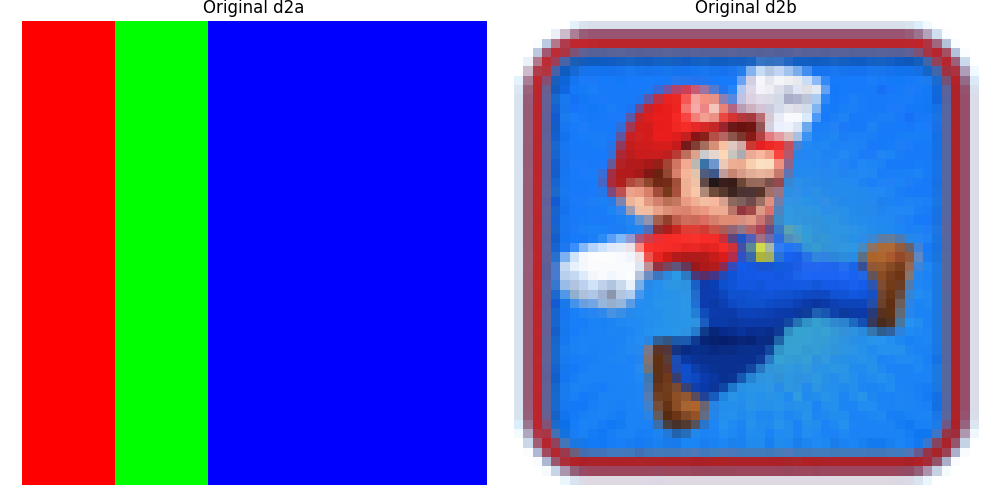
\includegraphics[width=0.8\textwidth]{original_images.png}
\caption{Οπτικοποίηση των εικόνων \en d2a \gr και \en d2b \gr από το αρχείο \en \texttt{dip\_hw\_3.mat}\gr.}
\end{figure}

\chapter{Εικόνες ως Γράφοι και \en Spectral Clustering\gr}

Σε αυτή την ενότητα περιγράφεται η θεμελιώδης ιδέα της μετατροπής μιας εικόνας σε γράφο, μια τεχνική απαραίτητη για την εφαρμογή αλγορίθμων φασματικής τμηματοποίησης όπως οι \en Spectral Clustering \gr και \en Normalized Cuts \gr αλλά και της τεχνικής \en Spectral Clustering\gr. Η υλοποίηση βασίζεται στην κατασκευή ενός πίνακα γειτνίασης \en (affinity matrix)\gr, όπου κάθε \en pixel \gr αποτελεί έναν κόμβο και οι ακμές μεταξύ τους αντανακλούν μετρικές ομοιότητας.

\vspace{0.4cm}

\section{Συνάρτηση για Εικόνα σε Γράφο}

Η μετάβαση από μια αναπαράσταση εικόνας σε γράφο αποτελεί απαραίτητο βήμα για την εφαρμογή φασματικών μεθόδων ομαδοποίησης, όπως \en Spectral Clustering \gr και \en Normalized Cuts\gr. Η συνάρτηση \en \texttt{image\_to\_graph()} \gr αναλαμβάνει να κατασκευάσει τον πίνακα γειτνίασης \en (affinity matrix) \gr που περιγράφει έναν μη-κατευθυντικό πλήρως συνδεδεμένο γράφο, όπου κάθε κόμβος αντιστοιχεί σε ένα \en pixel \gr της εικόνας.

\vspace{0.3cm}

\subsection{Θεωρητική Ανάλυση}

Έστω ότι η είσοδος είναι μια εικόνα \en \texttt{img\_array} \gr διαστάσεων $M \times N \times C$, όπου $C$ ο αριθμός των καναλιών (συνήθως $C = 3$ για έγχρωμες εικόνες \en RGB\gr). Η μετατροπή της εικόνας σε γράφο περιλαμβάνει τα εξής στάδια:

\begin{enumerate}
    \item \textit{Μετασχηματισμός των \en pixels \gr σε διανύσματα:} Κάθε \en pixel \gr θεωρείται σημείο $x_i \in \mathbb{R}^C$ (με $C$ χαρακτηριστικά). Η εικόνα επίπεδο-επιπέδου μετατρέπεται σε έναν πίνακα διαστάσεων $(MN) \times C$.
    
    \item \textit{Υπολογισμός αποστάσεων μεταξύ των \en pixels\gr:} Για κάθε ζεύγος κόμβων $(i,j)$ υπολογίζεται η Ευκλείδεια απόσταση μεταξύ των διανυσμάτων $x_i, x_j$ ως:
    \[
    d(i,j) = \|x_i - x_j\| = \sqrt{\|x_i\|^2 + \|x_j\|^2 - 2 x_i \cdot x_j}
    \]
    
    \item \textit{Κατασκευή του \en affinity matrix\gr:} Η ομοιότητα μεταξύ δύο κόμβων ορίζεται ως:
    \[
    A(i,j) = e^{-d(i,j)}
    \]
    Το αποτέλεσμα είναι ένας πλήρως συμμετρικός πίνακας $A \in \mathbb{R}^{MN \times MN}$ όπου κάθε τιμή εκφράζει την ομοιότητα μεταξύ δύο \en pixels\gr.

    \item \textit{Ιδιότητες πίνακα:} Ο πίνακας που κατασκευάζεται είναι:
    \begin{itemize}
        \item \textit{Πυκνός} \en (fully-connected) \gr
        \item \textit{Συμμετρικός} ($A = A^\top$)
        \item \textit{Θετικά ορισμένος} (καθώς $e^{-d(i,j)} > 0$ για κάθε $i,j$)
    \end{itemize}
\end{enumerate}

\vspace{0.3cm}

\subsection{Ανάλυση Κώδικα και Ψευδοκώδικας}

Η υλοποίηση βασίζεται στο παρακάτω διάγραμμα ψευδοκώδικα, που περιγράφει βήμα προς βήμα τη λογική της \en \texttt{image\_to\_graph()}\gr:

\begin{tcolorbox}[colback=gray!5!white, colframe=black!75!black, title=Ψευδοκώδικας \en \texttt{image\_to\_graph()}\gr]
\en
\begin{verbatim}
1. [M, N, C] ← shape(img_array)
2. pixels ← reshape(img_array) to shape (MN, C)

3. sq_norms ← row squared L2 norms of pixels (shape MN×1)

4. D_sq ← pairwise squared Euclidean distances:
          D_sq = sq_norms + sq_norms.T - 2 * pixels.dot(pixels.T)

5. D ← sqrt(max(D_sq, 0))   # numerical stability

6. affinity_mat ← exp(-D)   # similarity matrix

7. return affinity_mat
\end{verbatim}
\gr
\end{tcolorbox}

\vspace{0.2cm}

\hspace{-0.6cm}Η παραπάνω συνάρτηση κατασκευάζει επιτυχώς τον γράφο, ο οποίος στη συνέχεια χρησιμοποιείται από τις συναρτήσεις \en \texttt{spectral\_clustering()} \gr και \en \texttt{n\_cuts\_recursive()} \gr για την υλοποίηση της τμηματοποίησης εικόνας.

\vspace{0.2cm}
\hspace{-0.6cm}Ο αντίστοιχος κώδικας \en Python \gr βρίσκεται στο αρχείο \en \texttt{image\_to\_graph.py} \gr.

\vspace{0.5cm}

\section{Συνάρτηση για \en Spectral Clustering\gr}

Η φασματική ομαδοποίηση (\en Spectral Clustering\gr) βασίζεται στην ιδιοφασματική ανάλυση του πίνακα γειτνίασης (\en affinity matrix\gr) και επιτρέπει την εύρεση μη γραμμικά διαχωρίσιμων ομάδων. Η συνάρτηση \en \texttt{spectral\_clustering()} \gr υλοποιεί τα βασικά στάδια του αλγορίθμου που περιγράφονται στη θεωρία, με είσοδο έναν συμμετρικό \en affinity \gr πίνακα και έναν ακέραιο αριθμό \en clusters \gr $k$.

\vspace{0.3cm}

\subsection{Θεωρητική Ανάλυση}

Η μέθοδος \en Spectral Clustering \gr βασίζεται στην ιδιοφασματική ανάλυση του γράφου που περιγράφεται από τον πίνακα γειτνίασης (ή \en affinity matrix\gr) $W \in \mathbb{R}^{n \times n}$. Ο γράφος υποτίθεται ότι είναι μη-κατευθυντικός, πλήρως συνδεδεμένος και με θετικές ακμές.

\hspace{-0.6cm}Η διαδικασία περιλαμβάνει τα παρακάτω βήματα:

\begin{enumerate}
    \item \textit{Κατασκευή του διαγώνιου πίνακα βαθμού $D$:} 
    Ορίζεται ως:
    \[
    D(i,i) = \sum_j W(i,j), \quad D(i,j) = 0 \ \text{για } i \neq j
    \]
    Ο πίνακας $D$ περιέχει στον διαγώνιο την τιμή του βαθμού κάθε κόμβου (το άθροισμα των βαρών όλων των εισερχόμενων ακμών).

    \item \textit{Υπολογισμός Λαπλασιανού πίνακα $L$:} 
    Ο μη-κανονικοποιημένος \en Laplacian \gr δίνεται από:
    \[
    L = D - W
    \]
    Ο πίνακας $L$ είναι συμμετρικός και θετικά ημι-ορισμένος. Οι ιδιοτιμές του είναι μη αρνητικές, και η μικρότερη ιδιοτιμή είναι πάντα $0$ (με αντίστοιχο ιδιοδιάνυσμα το $\mathbf{1}$).

    \item \textit{Επίλυση του ιδιοτιμικού προβλήματος:}
    Λύνουμε το πρόβλημα:
    \[
    Lx = \lambda x
    \]
    και επιλέγουμε τα $k$ ιδιοδιανύσματα που αντιστοιχούν στις $k$ μικρότερες ιδιοτιμές (εκτός της μηδενικής, εφόσον είναι απομονωμένη). Αυτά περιέχουν τις πιο σημαντικές πληροφορίες σχετικά με τη δομή του γράφου.

    \item \textit{Κατασκευή πίνακα χαρακτηριστικών $U$:}
    Ορίζουμε τον πίνακα:
    \[
    U = [u_1 \, u_2 \, \dots \, u_k] \in \mathbb{R}^{n \times k}
    \]
    όπου κάθε στήλη είναι ένα από τα επιλεγμένα ιδιοδιανύσματα. Ο πίνακας $U$ θεωρείται ως νέα αναπαράσταση \en (embedding) \gr των κόμβων σε $k$-διάστατο χώρο.

    \item \textit{Ομαδοποίηση με \en k-means\gr:}
    Κάθε γραμμή του $U$ (δηλαδή κάθε κόμβος του γράφου) θεωρείται ως ένα $k$-διάστατο διάνυσμα $y_i \in \mathbb{R}^k$. Εφαρμόζεται ο αλγόριθμος \en k-means \gr στα $n$ σημεία $\{y_i\}_{i=1}^{n}$ ώστε να εκχωρηθεί κάθε κόμβος σε ένα από τα $k$ \en clusters\gr:
    \[
    C_1, C_2, \dots, C_k
    \]
\end{enumerate}

\vspace{0.3cm}

\subsection{Ανάλυση Κώδικα και Ψευδοκώδικας}

Η λογική του αλγορίθμου φαίνεται συγκεντρωτικά στον παρακάτω ψευδοκώδικα:

\begin{tcolorbox}[colback=gray!5!white, colframe=black!75!black, title=Ψευδοκώδικας \en \texttt{spectral\_clustering()}\gr]
\en
\begin{verbatim}
1. [n, _] ← shape(affinity_mat)
2. assert square matrix and k < n

3. W ← sparse CSR matrix from affinity_mat
4. W.setdiag(0)  # zero self-loops
5. D ← diagonal matrix of degrees: D(i) = sum_j W(i,j)

6. L ← D - W     # Laplacian

7. [vals, vecs] ← eigs(L, M=D, k=k, which='SM')
   U ← real(vecs)  # take real part if complex

8. kmeans ← KMeans(n_clusters=k, random_state=1)
9. kmeans.fit(U)
10. return kmeans.labels_.astype(float)
\end{verbatim}
\gr
\end{tcolorbox}

\vspace{0.3cm}

\hspace{-0.6cm}\textbf{Σημειώσεις Υλοποίησης:}
\begin{itemize}
    \item Η χρήση του παραμέτρου \en \texttt{which='SM'} \gr στην \en \texttt{scipy.sparse.linalg.eigs()} \gr ζητά τις $k$ ιδιοτιμές με το μικρότερο μέτρο.
    \item Ο \en Laplacian \gr μπορεί να είναι είτε ο κανονικός είτε ο κανονικοποιημένος. Εδώ επιλέγεται ο μη κανονικοποιημένος.
    \item Για λόγους αναπαραγωγιμότητας, το \en \texttt{random\_state} \gr του \en \texttt{KMeans} \gr ορίζεται ίσο με $1$.
\end{itemize}

\vspace{0.3cm}

\hspace{-0.6cm}Η παραπάνω συνάρτηση αποτελεί βασικό δομικό στοιχείο τόσο για την εφαρμογή \en Spectral Clustering \gr όσο και για την συγκριση που μας ζητείται αργότερα με την επαναληπτική εφαρμογή της μεθόδου για τμηματοποίηση εικόνας.

\vspace{0.2cm}
\hspace{-0.6cm}Ο αντίστοιχος κώδικας \en Python \gr βρίσκεται στο αρχείο \en \texttt{spectral\_clustering.py} \gr.

\vspace{0.5cm}

\section{Ανάλυση Αποτελεσμάτων και Οπτικοποίησης}

Σε αυτό το \en section \gr πρόκειται να αναδείξουμε τα αποτελέσματα που προέκυψαν από την εφαρμογή τον προεναφερθέντων υλοποιημένων συναρτήσεων στα αρχεία \en \texttt{demo1.py} \gr και \en \texttt{demo2.py}\gr.

\subsection{Περιγραφή και λειτουργικότητα \en demo1.py\gr}

Το αρχείο \en \texttt{demo1.py} \gr χρησιμοποιείται για την πειραματική επαλήθευση της λειτουργίας της συνάρτησης \en \texttt{spectral\_clustering()}\gr, όπως ορίζεται στην προηγούμενη \en section\gr. Ειδικότερα, φορτώνει τον \en affinity matrix \gr από το αρχείο \en \texttt{dip\_hw\_3.mat} \gr (μεταβλητή \en \texttt{d1a}\gr), εφαρμόζει φασματική ομαδοποίηση για τρεις διαφορετικές τιμές $k = 2, 3, 4$, και παρουσιάζει τα εξής:

\begin{itemize}
    \item Τις πρώτες 20 ετικέτες που παράγονται από την κλήση της \en \texttt{spectral\_clustering()} \gr για κάθε τιμή του $k$.
    \item Το μέγεθος κάθε \en cluster\gr, δηλαδή πόσα σημεία περιλαμβάνει.
    \item Δύο διαγράμματα για κάθε $k$:
    \begin{itemize}
        \item \textit{Διάγραμμα ετικετών}: Παρουσιάζει γραφικά τις πρώτες $20$ ετικέτες \en cluster \gr που εκχωρήθηκαν.
        \item \textit{Διάγραμμα μεγεθών}: Παρουσιάζει το μέγεθος κάθε \en cluster \gr υπό μορφή \en bar plot\gr.
    \end{itemize}
\end{itemize}

\hspace{-0.6cm}Η χρήση της παραμέτρου \en \texttt{random\_state = 1} \gr στη συνάρτηση \en \texttt{KMeans()} \gr εξασφαλίζει την αναπαραγωγή των αποτελεσμάτων σε κάθε εκτέλεση. Η επόμενη υποενότητα παραθέτει και σχολιάζει τα αποτελέσματα που προέκυψαν.

\vspace{0.3cm}

\subsubsection{Παράθεση Αποτελεσμάτων}

Η εκτέλεση του \en \texttt{demo1.py} \gr για τιμές \( k = 2, 3, 4 \) παρήγαγε τις παρακάτω ετικέτες και μεγέθη \en clusters\gr:

\begin{itemize}
    \item \textit{\( k = 2 \):}  
    \begin{itemize}
        \item Πρώτες 20 ετικέτες: \texttt{[1 1 1 1 0 0 0 0 0 0 0 0]}
        \item Μέγεθος \en clusters\gr: \texttt{[8 4]}
        \item \textit{Παρατήρηση:} Το σύνολο των 12 σημείων διαχωρίστηκε σε 2 ομάδες με σχετικά ανισοβαρή κατανομή.
    \end{itemize}

    \item \textit{\( k = 3 \):}  
    \begin{itemize}
        \item Πρώτες 20 ετικέτες: \texttt{[1 1 1 1 0 0 0 0 2 2 2 2]}
        \item Μέγεθος \en clusters\gr: \texttt{[4 4 4]}
        \item \textit{Παρατήρηση:} Η ομαδοποίηση είναι αρκετά ισορροπημένη, υποδεικνύοντας φυσικό διαχωρισμό των δεδομένων σε 3 ίσες κατηγορίες.
    \end{itemize}

    \item \textit{\( k = 4 \):}
    \begin{itemize}
        \item Πρώτες 20 ετικέτες: \texttt{[2 3 3 3 0 0 0 0 1 1 1 1]}
        \item Μέγεθος \en clusters\gr: \texttt{[4 4 1 3]}
        \item \textit{Παρατήρηση:} Ο διαχωρισμός είναι πιο ανισοβαρής, με ένα \en cluster \gr που περιλαμβάνει μόνο ένα σημείο. Αυτό μπορεί να υποδεικνύει υπερδιάσπαση για \( k = 4 \).
    \end{itemize}
\end{itemize}

\vspace{0.4cm}
\hspace{-0.6cm}Τα αποτελέσματα δείχνουν πως η επιλογή του αριθμού των \en clusters \gr \( k \) επηρεάζει σημαντικά τη σταθερότητα και την ισορροπία της ομαδοποίησης. Η περίπτωση \( k=3 \) φαίνεται να προσφέρει την πιο συνεκτική κατανομή.

\vspace{0.5cm}
\hspace{-0.6cm}Παρακάτω παρουσιάζονται ενδεικτικά γραφήματα των πρώτων ετικετών καθώς και τα μεγέθη των \en clusters\gr:

\begin{figure}[H]
    \centering
    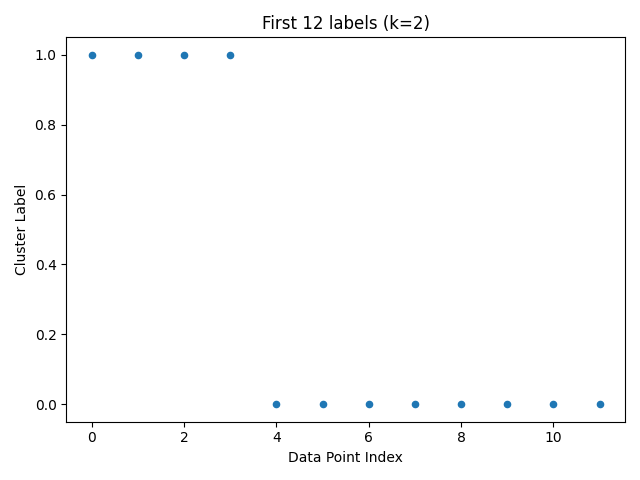
\includegraphics[width=0.45\textwidth]{demo1_k2_first_labels.png}
    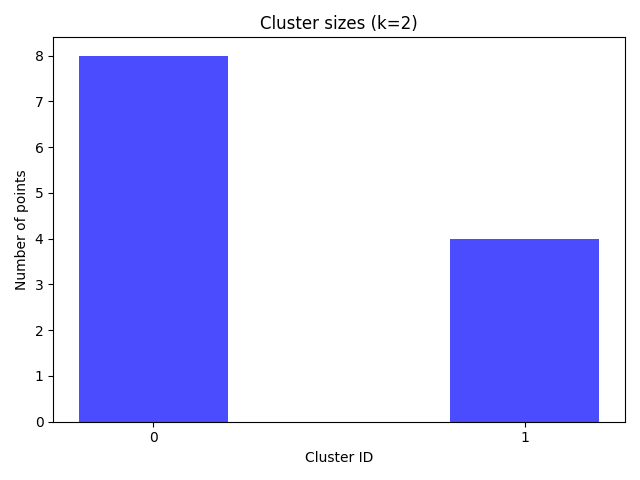
\includegraphics[width=0.45\textwidth]{demo1_k2_cluster_sizes.png}
    \caption{Ετικέτες και μεγέθη \en clusters \gr για \(\mathbf{k=2}\)}
\end{figure}

\begin{figure}[H]
    \centering
    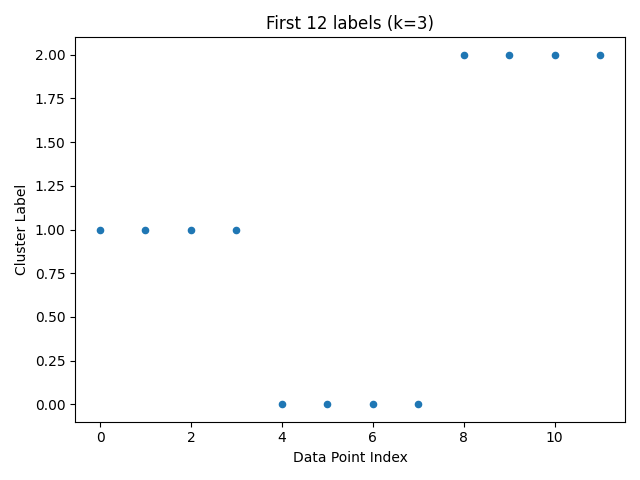
\includegraphics[width=0.45\textwidth]{demo1_k3_first_labels.png}
    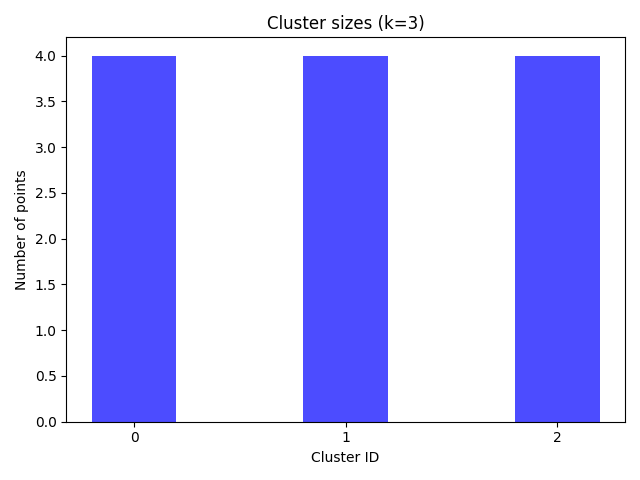
\includegraphics[width=0.45\textwidth]{demo1_k3_cluster_sizes.png}
    \caption{Ετικέτες και μεγέθη \en clusters \gr για \(\mathbf{k=3}\)}
\end{figure}

\begin{figure}[H]
    \centering
    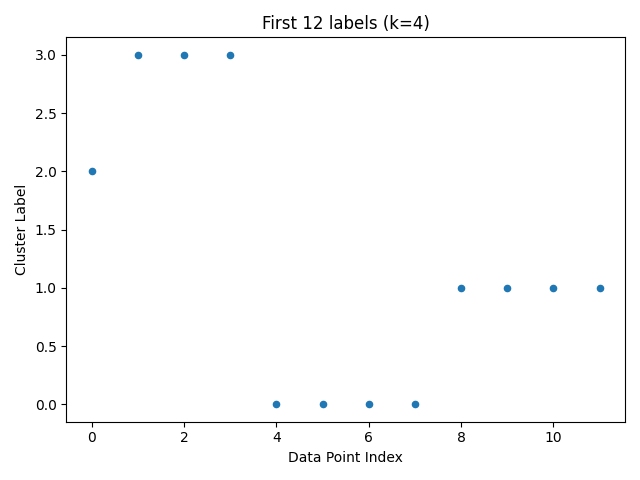
\includegraphics[width=0.45\textwidth]{demo1_k4_first_labels.png}
    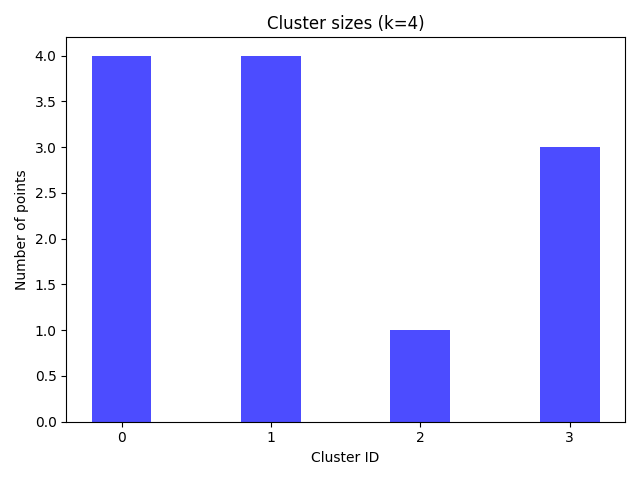
\includegraphics[width=0.45\textwidth]{demo1_k4_cluster_sizes.png}
    \caption{Ετικέτες και μεγέθη \en clusters \gr για \(\mathbf{k=4}\)}
\end{figure}

\newpage

\subsection{Περιγραφή και λειτουργικότητα \en demo2.py\gr}

Το αρχείο \en \texttt{demo2.py} \gr αξιοποιεί τη συνάρτηση \en \texttt{spectral\_clustering()} \gr σε συνδυασμό με τη \en \texttt{image\_to\_graph()} \gr για την τμηματοποίηση πραγματικών εικόνων. Συγκεκριμένα:

\begin{itemize}
    \item Φορτώνονται από το \en \texttt{dip\_hw\_3.mat} \gr οι δύο έγχρωμες εικόνες \en \texttt{d2a} \gr και \en \texttt{d2b} \gr.
    \item Κάθε εικόνα μετατρέπεται σε γράφο μέσω της \en \texttt{image\_to\_graph()} \gr (παράγοντας τον \en affinity matrix \gr).
    \item Εκτελείται φασματική ομαδοποίηση για τρεις διαφορετικές τιμές $k = 2, 3, 4$.
    \item Οι τελικές ετικέτες \en cluster \gr αναδιαμορφώνονται σε εικόνες, και απεικονίζονται με χρωματική κωδικοποίηση (χάρτης χρωμάτων \en jet\gr).
\end{itemize}

\hspace{-0.6cm}Για κάθε εικόνα, αποθηκεύεται ένα αρχείο μορφής \en PNG \gr που περιέχει τις τρεις τμηματοποιήσεις με βάση τις τιμές του $k$. Οι εικόνες αποθηκεύονται με ονόματα \en \texttt{d2a\_segmentation.png} \gr και \en \texttt{d2b\_segmentation.png} \gr.

\vspace{0.3cm}

\subsubsection{Παράθεση Αποτελεσμάτων}

Οι τελικές εικόνες που προέκυψαν από τη διαδικασία \en spectral clustering \gr παρουσιάζονται παρακάτω. Κάθε εικόνα περιλαμβάνει τις τρεις τμηματοποιήσεις για $k = 2, 3, 4$:

\begin{figure}[H]
    \centering
    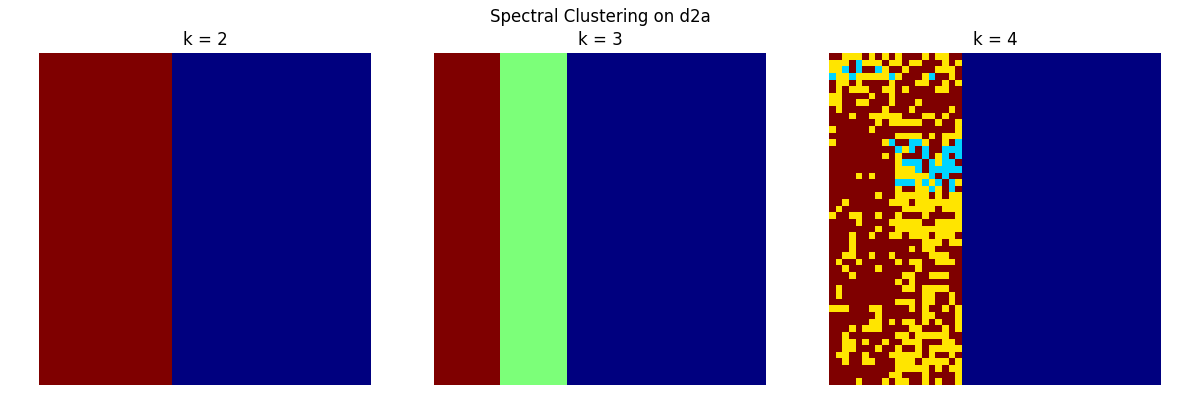
\includegraphics[width=0.95\textwidth]{d2a_segmentation.png}
    \caption{Τμηματοποίηση εικόνας \en d2a \gr για $k = 2, 3, 4$}
\end{figure}

\begin{figure}[H]
    \centering
    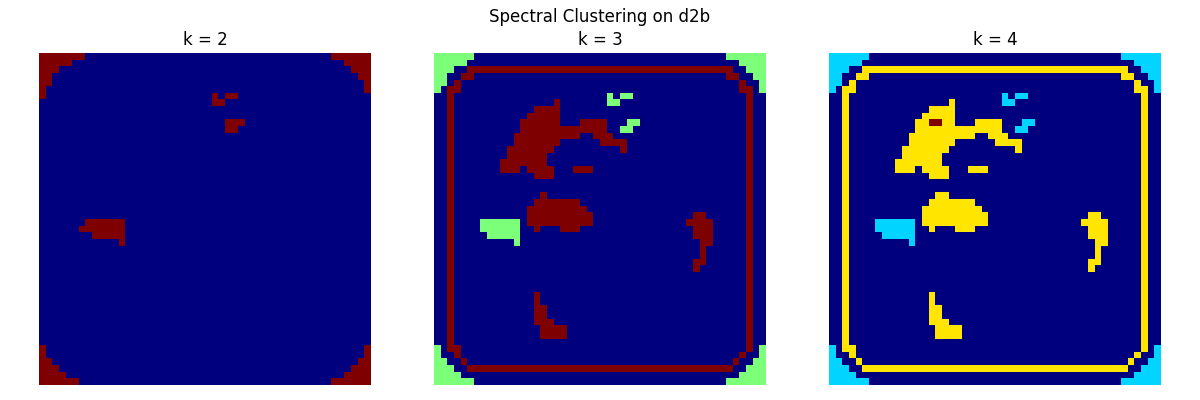
\includegraphics[width=0.95\textwidth]{d2b_segmentation.png}
    \caption{Τμηματοποίηση εικόνας \en d2b \gr για $k = 2, 3, 4$}
\end{figure}

\vspace{0.3cm}
\hspace{-0.6cm}Η επιλογή διαφορετικών τιμών για $k$ οδηγεί σε εμφανώς διαφορετική κατανομή των περιοχών της εικόνας. Για παράδειγμα, μικρές τιμές όπως $k=2$ δίνουν γενικές κατηγορίες, ενώ μεγαλύτερες τιμές $k=4$ οδηγούν σε πιο λεπτομερή διαχωρισμό, αλλά ενδέχεται να προκύψουν υπερ-τμηματοποιήσεις.

\vspace{0.3cm}
\hspace{-0.6cm}Η παράμετρος \en \texttt{random\_state = 1} \gr εξασφαλίζει ότι η τυχαία αρχικοποίηση του \en k-means \gr δίνει αναπαραγώγιμα αποτελέσματα ανά εκτέλεση.

\subsubsection{Παρατηρήσεις και Συμπεράσματα}

\begin{itemize}
    \item \textit{Εικόνα \en \texttt{d2a}\gr:} Η φασματική ομαδοποίηση αποδίδει άριστα για $k=2$ και $k=3$, καταφέρνοντας να εντοπίσει τις μεγάλες χρωματικές περιοχές. Για $k=4$, προκύπτουν ανεπιθύμητα μικρά θορυβώδη \en clusters\gr, φανερώνοντας ότι η τιμή αυτή μπορεί να είναι υπερβολική για τη συγκεκριμένη εικόνα.
    
    \item \textit{Εικόνα \en \texttt{d2b}\gr:} Πρόκειται για πολύπλοκη εικόνα, με υψηλή παραμόρφωση και πολλά αντικείμενα. Παρατηρείται:
    \begin{itemize}
        \item Για $k=2$: περιορισμένη τμηματοποίηση.
        \item Για $k=3$: σημαντική βελτίωση με ανίχνευση περιγραμμάτων.
        \item Για $k=4$: εμφανίζονται επιμέρους λεπτομέρειες, ωστόσο κάποια \en clusters \gr είναι υπερβολικά τοπικά.
    \end{itemize}

    \item Η μέθοδος \en \texttt{spectral\_clustering} \gr είναι ιδιαίτερα αποτελεσματική για εικόνες με καθαρή δομή (π.χ. \en \texttt{d2a}\gr). Αντίθετα, σε περιπτώσεις σύνθετων και θορυβωδών εικόνων (όπως η \en \texttt{d2b}\gr), η επιλογή της παραμέτρου $k$ παίζει κρίσιμο ρόλο στην ποιότητα του αποτελέσματος.

    \item Η αλλαγή  πίνακα γειτνίασης \en (affinity matrix) \gr θα έπαιζε καθοριστικό ρόλο προκειμένου να μπορούσαμε να διακρίνουμε αισθητές βελτιώσεις.
\end{itemize}

\vspace{0.2cm}
\hspace{-0.6cm}Οι αντίστοιχοι κώδικες \en Python \gr βρίσκονται στα αρχεία \en \texttt{demo1.py} \gr και \en \texttt{demo2.py} \gr.

\chapter{Μέθοδοι \en Normalized-cuts\gr}

Η μέθοδος \en Normalized-cuts (n-cuts) \gr αποτελεί μια προχωρημένη τεχνική τμηματοποίησης εικόνων βασισμένη στη θεωρία γράφων. Σε αντίθεση με απλούστερες μεθόδους όπως το \en spectral clustering\gr, λαμβάνει υπόψη όχι μόνο τη συνοχή εντός των \en clusters \gr αλλά και τη σχετική ανεξαρτησία μεταξύ τους. Στο κεφάλαιο αυτό θα παρουσιαστούν τόσο η μη-αναδρομική όσο και η αναδρομική υλοποίηση της μεθόδου, συνοδευόμενες από αριθμητικά παραδείγματα και πειραματικά αποτελέσματα.

\section{Μέθοδος \en n-cuts\gr}

Οπως προαναφέρθηκε η μέθοδος \en n-cuts \gr αποτελεί επέκταση του \en spectral clustering \gr και επιδιώκει την εύρεση μιας βέλτιστης διχοτόμησης ενός γράφου ελαχιστοποιώντας μια σχετική μετρική \en Ncut\gr. Η παρακάτω ενότητα περιγράφει αναλυτικά τόσο την υπολογιστική διαδικασία εξαγωγής των ομάδων (μέσω του ιδιοπροβλήματος), όσο και τον ακριβή υπολογισμό της τιμής της μετρικής \en Ncut \gr για δεδομένη διχοτόμηση.

\vspace{0.4cm}

\subsection{Υλοποίηση ομαδοποίησης με τη \en \texttt{n\_cuts()}\gr}

Η συνάρτηση \en \texttt{n\_cuts()} \gr αποτελεί την υλοποίηση της μη αναδρομικής εκδοχής της μεθόδου \en normalized cuts\gr, βασισμένης στη φασματική ανάλυση του Λαπλασιανού πίνακα του γράφου. Πιο συγκεκριμένα, δέχεται ως είσοδο έναν πίνακα γειτνίασης \en (affinity matrix) \gr και έναν αριθμό ομάδων $k$ και επιστρέφει διανύσματα ετικετών για τα $n$ σημεία.

Η μέθοδος πραγματοποιεί τα εξής στάδια:

\begin{enumerate}
    \item Αρχικά μετατρέπει τον πίνακα \en \texttt{affinity\_mat} \gr σε αραιό πίνακα \en (sparse format)\gr, και μηδενίζει τη διαγώνιο ώστε να εξαλειφθούν οι αυτοσυνδέσεις \en (self-loops)\gr.
    \item Υπολογίζει το διαγώνιο πίνακα βαθμών \( D \), όπου κάθε τιμή \( D_{ii} = \sum_j W_{ij} \), και κατασκευάζει τον μη-κανονικοποιημένο Λαπλασιανό \( L = D - W \).
    \item Λύνει το γενικευμένο ιδιοπρόβλημα \( L \mathbf{v} = \lambda D \mathbf{v} \) για τις $k$ ιδιοτιμές με τη μικρότερη απόλυτη τιμή, μέσω της συνάρτησης \en \texttt{eigs()} \gr του πακέτου \en \texttt{scipy}\gr.
    \item Χρησιμοποιεί τα $k$ ιδιοδιανύσματα που προκύπτουν (συναποτελούν τον πίνακα \( U \in \mathbb{R}^{n \times k} \)) ως νέα χαρακτηριστικά σημεία, και εκτελεί \en k-means clustering \gr σε αυτά, ώστε να παραχθούν οι τελικές ομάδες.
\end{enumerate}

\vspace{0.3cm}
\noindent \textbf{Παρατήρηση:} Στην προεπιλεγμένη του λειτουργία, ο υπολογισμός των ιδιοδιανυσμάτων μέσω της \en \texttt{eigs()} \gr εμπεριέχει εσωτερική στοχαστικότητα \en (random initialization \gr μέσω \en Lanczos iteration\gr). Για την εξασφάλιση αναπαραγώγιμων αποτελεσμάτων, μπορεί να δοθεί συγκεκριμένο αρχικό διάνυσμα \( v_0 \neq 0 \), όπως στο παρακάτω (σχολιασμένο) απόσπασμα του κώδικα:
\vspace{0.3cm}

\en
\begin{lstlisting}[language=Python]
# --> For deterministic results, use a fixed nonzero vector as v0
n = L.shape[0]
v0 = np.ones(n)
vals, vecs = eigs(L, M=D, k=k, which='SM', v0=v0)
\end{lstlisting}
\gr
\vspace{0.3cm}

\hspace{-0.6cm}Η πρακτική αυτή θα μπορούσε να είναι ιδιαίτερα σημαντική για συνεπή συγκριτική αξιολόγηση των αποτελεσμάτων σε πειραματικές μελέτες ωστόσο δεν χρησιμοποιήθηκε για την εξαγωγή αποτελεσμάτων στην γενικότερη υλοποίηση της εργασίας.

\hspace{-0.6cm}Ακολουθεί ψευδοκώδικας που αναπαριστά τον συλλογισμό μου στην δόμηση του κώδικα:

\begin{tcolorbox}[colback=gray!5!white, colframe=black!75!black, title=Ψευδοκώδικας \en \texttt{n\_cuts()}\gr]
\en
\begin{verbatim}
1. W ← csr_matrix(affinity_mat); set W[i,i] ← 0
2. D ← diagonal matrix with row sums of W
3. L ← D - W
4. [vals, vecs] ← eigs(L, M=D, k=k)
5. U ← real(vecs)
6. Cluster rows of U with KMeans(n_clusters=k)
7. Return cluster labels
\end{verbatim}
\gr
\end{tcolorbox}

\vspace{0.5cm}

\subsection{Υπολογισμός της μετρικής \en \texttt{Ncut(A,B)}\gr}

Η πραγματική τιμή της μετρικής \en \texttt{Ncut(A,B)} \gr για δεδομένο διαχωρισμό σε δύο ομάδες υπολογίζεται με τη συνάρτηση \en \texttt{calculate\_n\_cut\_value()}\gr. Η μετρική δίνεται από:
\en
\[
\text{Ncut}(A,B) = 2 - \left( \frac{\text{assoc}(A,A)}{\text{assoc}(A,V)} + \frac{\text{assoc}(B,B)}{\text{assoc}(B,V)} \right)
\]
\en 
\begin{itemize}
    \item \(\text{assoc}(A,V) = \sum_{i \in A, j \in V} W(i,j)\)
    \item \(\text{assoc}(A,A) = \sum_{i,j \in A} W(i,j)\)
    \item \gr Ομοίως για \en \(B\)
\end{itemize}
\gr

\hspace{-0.6cm}Αυτός ο υπολογισμός είναι χρήσιμος ειδικά σε ιεραρχικές ή αναδρομικές στρατηγικές (π.χ. \en \texttt{n\_cuts\_recursive}\gr) που θα αναδειχθεί ως υλοποίηση σε επόμενο \en section\gr, ώστε να ελέγχεται αν μια διχοτόμηση είναι αρκετά καλή με βάση κάποιο κατώφλι \(T_2\).

\vspace{0.3cm}

\hspace{-0.6cm}Ακολουθεί ψευδοκώδικας που αναπαριστά τον συλλογισμό μου στην δόμηση του κώδικα για την συνάρτηση \en \texttt{calculate\_n\_cut\_value()}\gr:

\begin{tcolorbox}[colback=gray!5!white, colframe=black!75!black, title=Ψευδοκώδικας \en \texttt{calculate\_n\_cut\_value()}\gr]
\en
\begin{verbatim}
1. A ← indices of cluster 0
   B ← indices of cluster 1

2. assoc_A_V ← sum of W[i,:] for i in A
   assoc_B_V ← sum of W[i,:] for i in B

3. assoc_A_A ← sum of W[i,j] for i,j in A
   assoc_B_B ← sum of W[i,j] for i,j in B

4. nassoc ← (assoc_A_A / assoc_A_V) + (assoc_B_B / assoc_B_V)
5. Return ncut_value ← 2 - nassoc
\end{verbatim}
\gr
\end{tcolorbox}

\vspace{0.5cm}

\section{Μέθοδος \en n-cuts Recursive\gr}

Η μέθοδος \en recursive n-cuts \gr αποτελεί μια αναδρομική παραλλαγή της φασματικής τεχνικής \en normalized cuts\gr, και στοχεύει στην επαναληπτική διάσπαση του γράφου σε υποσύνολα, με βάση ένα φασματικό κριτήριο ποιότητας (το \en normalized cut value\gr).

\vspace{0.2cm}

\hspace{-0.6cm}Η βασική ιδέα είναι να εφαρμόζεται το \en \texttt{n\_cuts()} \gr για \(k = 2\) και, ανάλογα με την ποιότητα του διαχωρισμού, να αποφασίζεται εάν η ομάδα πρέπει να διασπαστεί περαιτέρω ή να παραμείνει ως έχει.

\vspace{0.3cm}
\hspace{-0.6cm}Η συνάρτηση \en \texttt{n\_cuts\_recursive()} \gr βασίζεται στις συναρτήσεις \en \texttt{calculate\_n\_cut\_value()} \gr και \en \texttt{n\_cuts()} \gr που παρουσιάστηκαν στην προηγούμενη ενότητα. Η λογική της αναλυτικά:

\begin{itemize}
    \item Κρατά έναν πίνακα υποομάδων (\en \texttt{queue}\gr) που πρόκειται να εξεταστούν.
    \item Για κάθε ομάδα:
    \begin{itemize}
        \item Αν το μέγεθός της είναι μικρότερο από ένα κατώφλι \(T_1\), δεν διασπάται περαιτέρω.
        \item Αλλιώς, εφαρμόζεται η \en \texttt{n\_cuts()} \gr για \(k = 2\) ώστε να παραχθεί ένας δυαδικός διαχωρισμός.
        \item Υπολογίζεται η τιμή \en \texttt{Ncut} \gr με χρήση της \en \texttt{calculate\_n\_cut\_value()}\gr.
        \item Αν η τιμή αυτή ξεπερνά το κατώφλι \(T_2\), η ομάδα δεν διασπάται περαιτέρω.
        \item Διαφορετικά, διαχωρίζεται στις δύο υποομάδες και αυτές επιστρέφουν στην \en \texttt{queue}\gr.
    \end{itemize}
    \item Η διαδικασία συνεχίζεται έως ότου καμία υποομάδα να μην μπορεί ή να μην πρέπει να διασπαστεί περαιτέρω.
\end{itemize}

\vspace{0.4cm}
\hspace{-0.6cm}Ο τελικός πίνακας ετικετών (\en \texttt{cluster\_idx}\gr) επιστρέφει τις ομαδοποιήσεις όλων των κόμβων, όπως προέκυψαν από τη διαδικασία αναδρομικής διάσπασης.

\newpage

\vspace{0.4cm}
\noindent \textbf{Σχόλια και Πλεονεκτήματα:}
\begin{itemize}
    \item Η αναδρομική έκδοση επιτρέπει δυναμικό προσδιορισμό του αριθμού των τελικών ομάδων, ανάλογα με την τοπική δομή του γράφου.
    \item Ο συνδυασμός των κατωφλίων \(T_1\) (ελάχιστο πλήθος κόμβων) και \(T_2\) (ποιότητα διαχωρισμού) προσφέρει έλεγχο στο βάθος και στην ποιότητα της τμηματοποίησης.
    \item Ο αλγόριθμος είναι ιδιαίτερα χρήσιμος για προβλήματα \en image segmentation\gr, όπου δεν είναι εκ των προτέρων γνωστός ο αριθμός των αντικειμένων.
\end{itemize}

\vspace{0.4cm}
\noindent \textbf{Σημείωση:} Η απόδοση της συνάρτησης εξαρτάται άμεσα από την ποιότητα των \en affinity matrices \gr και την ορθή ρύθμιση των παραμέτρων \(T_1\) και \(T_2\). Μικρό \(T_2\) οδηγεί σε υπερδιάσπαση, ενώ μεγάλο μπορεί να αποτρέψει χρήσιμους διαχωρισμούς.

\vspace{0.3cm}

\hspace{-0.6cm}Παρακάτω παρατίθεται και ο αντίστοιχος Ψευδοκώδικας για την συνάρτηση \en \texttt{n\_cuts\_recursive()}\gr:

\begin{tcolorbox}[colback=gray!5!white, colframe=black!75!black, title=Ψευδοκώδικας \en \texttt{n\_cuts\_recursive()} \gr]
\en
\begin{verbatim}
1. Initialize queue ← [all node indices]
2. final_clusters ← []

3. While queue not empty:
    a. idx ← queue.pop(0)
    b. If len(idx) ≤ T1:
           final_clusters.append(idx)
           continue
    c. W_sub ← affinity_mat[idx, idx]
    d. labels ← n_cuts(W_sub, k=2)
    e. ncut_val ← calculate_n_cut_value(W_sub, labels)
    f. If ncut_val ≥ T2:
           final_clusters.append(idx)
       Else:
           part0 ← idx[labels == 0]
           part1 ← idx[labels == 1]
           queue.append(part0)
           queue.append(part1)

4. Assign final label to each group in final_clusters
5. Return cluster_idx
\end{verbatim}
\gr
\end{tcolorbox}

\newpage	

\section{Ανάλυση Αποτελεσμάτων και Οπτικοποίησης}

Σε αυτό το \en section \gr παρουσιάζονται και σχολιάζονται τα αποτελέσματα που προέκυψαν από την εφαρμογή των συναρτήσεων \en \texttt{n\_cuts()}, \texttt{calculate\_n\_cut\_value()} \gr και \en \texttt{n\_cuts\_recursive()} \gr στα scripts \en \texttt{demo3a.py}, \texttt{demo3b.py} \gr και \en \texttt{demo3c.py}\gr.

\vspace{0.2cm}

\hspace{-0.6cm}Η κάθε υποενότητα αναλύει τη λειτουργία της αντίστοιχης ρουτίνας, καθώς και τα αποτελέσματα που παράγονται για τις εικόνες \en \texttt{d2a} \gr και \en \texttt{d2b} \gr από το \en dataset\gr. Η σύγκριση με τη μέθοδο \en spectral clustering \gr δίνει καλύτερη εικόνα της συμπεριφοράς των υλοποιήσεων \en n-cuts\gr.

\subsection{Περιγραφή και λειτουργικότητα \en demo3a.py\gr}

Το αρχείο \en \texttt{demo3a.py} \gr αξιοποιεί τη μη-αναδρομική εκδοχή της μεθόδου \en n-cuts\gr για να ομαδοποιήσει τις εικόνες \en \texttt{d2a} \gr και \en \texttt{d2b}\gr, οι οποίες φορτώνονται από το αρχείο \en \texttt{dip\_hw\_3.mat}\gr. Για κάθε εικόνα, ακολουθούνται τα εξής βήματα:

\begin{itemize}
    \item Μετατροπή της εικόνας σε γράφο μέσω της συνάρτησης \en \texttt{image\_to\_graph()} \gr, ώστε να προκύψει ο \en affinity matrix \gr \(W\).
    \item Εκτέλεση της συνάρτησης \en \texttt{n\_cuts()} \gr για τρεις διαφορετικές τιμές αριθμού ομάδων: \(k = 2, 3, 4\).
    \item Ανακατασκευή των ετικετών σε μορφή εικόνας (πίνακας \(M \times N\)) και απεικόνιση των αποτελεσμάτων.
    \item Εκτύπωση του πλήθους των κόμβων σε κάθε \en cluster \gr για αξιολόγηση της ισορροπίας των αποτελεσμάτων.
\end{itemize}

\vspace{0.2cm}
\hspace{-0.6cm}Για κάθε μία από τις δύο εικόνες, παράγονται τρία διαγράμματα που αντιστοιχούν στις τιμές του \(k\). Τα αποτελέσματα αποθηκεύονται σε εικόνες με ονόματα τύπου \en \texttt{d2a\_n\_cuts.png} \gr και \en \texttt{d2b\_n\_cuts.png}\gr.

\subsubsection{Παράθεση Αποτελεσμάτων}

Παρακάτω παρατίθενται και τα αποτελέσματα του \en \texttt{demo3a.py}\gr.
 
\begin{figure}[H]
    \centering
    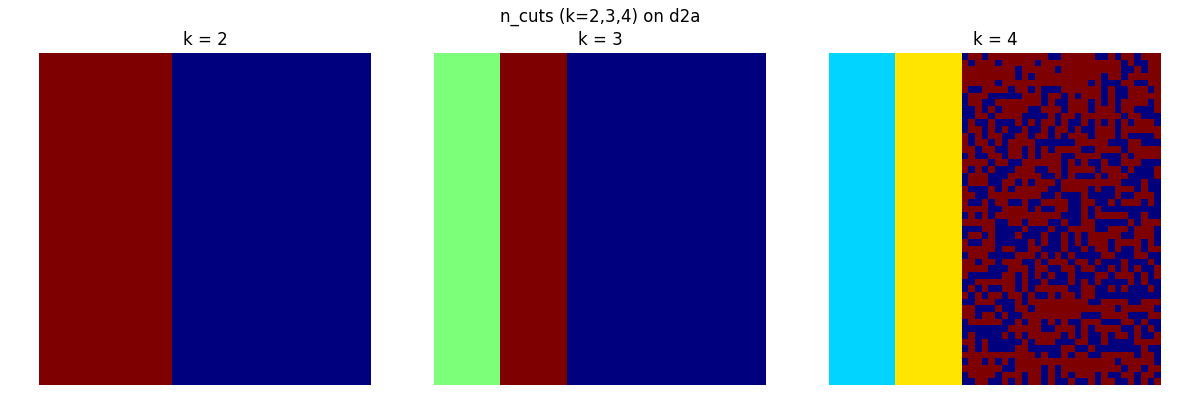
\includegraphics[width=0.95\textwidth]{d2a_n_cuts.png}
    \caption{Αποτελέσματα \en n-cuts \gr για \( \texttt{\en d2a \gr} \) με \( k=2,3,4 \)}
\end{figure}

\begin{figure}[H]
    \centering
    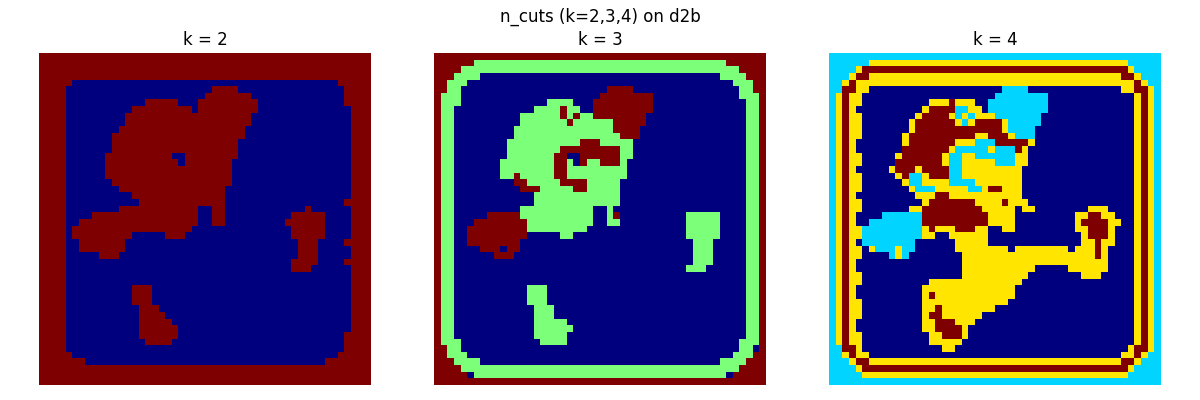
\includegraphics[width=0.95\textwidth]{d2b_n_cuts.png}
    \caption{Αποτελέσματα \en n-cuts \gr για \( \texttt{\en d2b \gr} \) με \( k=2,3,4 \)}
\end{figure}

\vspace{0.3cm}
\noindent Τα αντίστοιχα μεγέθη των \en clusters \gr που προέκυψαν από την εκτέλεση είναι:

\begin{itemize}
    \item \textit{}{Εικόνα \en \texttt{d2a}\gr}:
    \begin{itemize}
        \item \(k = 2:\) \texttt{[1500, 1000]}
        \item \(k = 3:\) \texttt{[1500, 500, 500]}
        \item \(k = 4:\) \texttt{[624, 500, 500, 876]}
    \end{itemize}

    \item \textit{}{Εικόνα \en \texttt{d2b}\gr}:
    \begin{itemize}
        \item \(k = 2:\) \texttt{[1360, 1140]}
        \item \(k = 3:\) \texttt{[1456, 659, 385]}
        \item \(k = 4:\) \texttt{[1028, 381, 752, 339]}
    \end{itemize}
\end{itemize}

\vspace{0.3cm}
\subsubsection{Σχολιασμός Αποτελεσμάτων}

Οι παρατηρήσεις που προκύπτουν είναι οι εξής:

\hspace{-0.6cm}\textbf{Για την εικόνα \en d2a:}
\begin{itemize}
    \item Με \(k = 2\): Δύο καθαρές, μεγάλες περιοχές (1500 και 1000 \en pixels\gr). Η τμηματοποίηση είναι ισχυρή και αναπαριστά το απλό μοτίβο της εικόνας.
    \item Με \(k = 3\): Το μεγάλο \en cluster \gr παραμένει σταθερό (1500 \en pixels\gr), ενώ εμφανίζονται δύο μικρότερα, συμμετρικά (500+500).
    \item Με \(k = 4\): Οι δύο περιοχές των 500 \en pixels \gr παραμένουν και εμφανίζονται δύο νέες (624 και 876), δείχνοντας ότι η μέθοδος διαχωρίζει επιπλέον λεπτομέρειες — με ενδεχόμενη υπερδιάσπαση.
\end{itemize}

\hspace{-0.6cm}\textbf{Για την εικόνα \en d2b:}
\begin{itemize}
    \item Με \(k = 2\): Σχετικά ισορροπημένος διαχωρισμός (1360–1140). Η τμηματοποίηση είναι απλοϊκή για την πολυπλοκότητα της εικόνας.
    \item Με \(k = 3\): Μεγαλύτερη διαφοροποίηση, με το κυρίαρχο \en cluster \gr να έχει 1456 \en pixels\gr. Ενδείξεις για καλύτερη αναγνώριση διαφορετικών περιοχών του αντικειμένου.
    \item Με \(k = 4\): Σημαντικά περισσότερη λεπτομέρεια. Το μέγεθος των \en clusters \gr είναι πιο ανισοβαρές, αλλά αποτυπώνουν διάφορες λειτουργικές περιοχές του αντικειμένου.
\end{itemize}

\vspace{0.3cm}
\hspace{-0.6cm}\textbf{Συμπεράσματα:}
\begin{itemize}
    \item Οι αριθμητικές τιμές των \en clusters \gr επιβεβαιώνουν τις παρατηρήσεις από τις οπτικοποιήσεις.
    \item Η εικόνα \en \texttt{d2a} \gr δείχνει σταθερότητα στις ομαδοποιήσεις καθώς αυξάνει το \(k\), ενώ η \en \texttt{d2b} \gr επωφελείται από μεγαλύτερο \(k\) για καλύτερη αποτύπωση της πολυπλοκότητας.
    \item Τέλος, για τη σύγκριση με την υλοποίηση της μεθόδου \en Spectral Clustering\gr, παρατηρούμε ότι η μέθοδος \en n-cuts\gr παρέχει σαφώς πιο καθαρά και λειτουργικά αποτελέσματα στην εικόνα \texttt{d2b}, ειδικά για μεγαλύτερες τιμές του \en k\gr. Οι δομές του αντικειμένου εντοπίζονται με μεγαλύτερη ακρίβεια και οι τμηματοποιήσεις διαχωρίζουν με σαφήνεια τα λειτουργικά μέρη του σχήματος. Αντίθετα, στην περίπτωση της εικόνας \en \texttt{d2a}\gr, για μικρές τιμές του \en k \gr (π.χ. \(k=2,3\)), και οι δύο μέθοδοι εμφανίζουν σχεδόν ταυτόσημα και οπτικά καθαρά αποτελέσματα. Ωστόσο, για \(k=4\), η μέθοδος \en Spectral Clustering \gr οδηγεί σε περισσότερη τυχαία κατανομή και θόρυβο, σε αντίθεση με την \en n-cuts\gr που, παρότι παρουσιάζει υπερδιάσπαση, διατηρεί πιο συνεπή και συστηματική τμηματοποίηση. Συνολικά, η \en n-cuts \gr εμφανίζεται πιο σταθερή και πιο αποτελεσματική, ιδίως σε περιπτώσεις σύνθετης δομής όπως στην \en \texttt{d2b}\gr.
\end{itemize}

\vspace{0.3cm}

\subsection{Περιγραφή και λειτουργικότητα \en demo3b.py\gr}

Το αρχείο \en \texttt{demo3b.py} \gr εξετάζει τη λειτουργία της μη-αναδρομικής μεθόδου \en n-cuts \gr για $k=2$, εφαρμόζοντας μόνο ένα βήμα διάσπασης στον αρχικό γράφο της εικόνας. Δηλαδή, η εικόνα διαχωρίζεται σε δύο υποσύνολα χωρίς περαιτέρω αναδρομή.

\hspace{-0.6cm}Η διαδικασία έχει ως εξής:
\begin{itemize}
    \item Για κάθε εικόνα \en \texttt{d2a}, \texttt{d2b}\gr, δημιουργείται ο \en affinity matrix \gr μέσω της \en \texttt{image\_to\_graph()}\gr.
    \item Εκτελείται η \en \texttt{n\_cuts()} \gr για \(k=2\).
    \item Υπολογίζεται η τιμή του \en \texttt{normalized cut} \gr μέσω της \en \texttt{calculate\_n\_cut\_value()}\gr.
    \item Τα αποτελέσματα αποθηκεύονται ως εικόνες και αναδεικνύονται παρακάτω.
\end{itemize}

\subsubsection{Παράθεση Αποτελεσμάτων}

Τα παρακάτω διαγράμματα παρουσιάζουν την οπτικοποίηση των διαχωρισμών:

\begin{figure}[H]
    \centering
    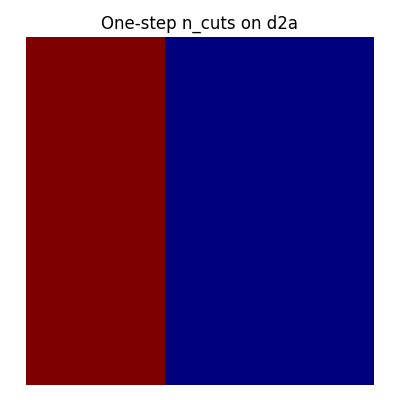
\includegraphics[width=0.35\textwidth]{d2a_one_step_n_cuts.png}
    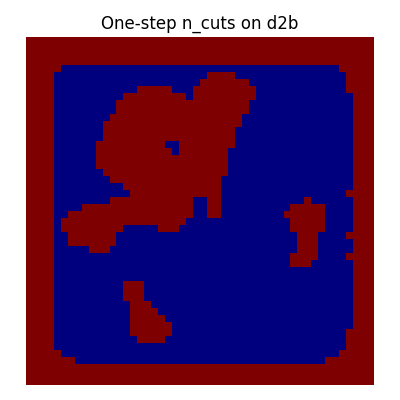
\includegraphics[width=0.35\textwidth]{d2b_one_step_n_cuts.png}
    \caption{Αποτελέσματα \en one-step n-cuts \gr για \en \texttt{d2a} \gr και \en \texttt{d2b} \gr με \(k=2\)}
\end{figure}

\vspace{0.3cm}
Οι αριθμοί και οι τιμές \en \texttt{Ncut} \gr για κάθε εικόνα είναι:

\begin{itemize}
    \item \textit{Εικόνα \en d2a\gr}:
    \begin{itemize}
        \item Μέγεθος \en clusters\gr: \texttt{[1500, 1000]}
        \item Τιμή \en \texttt{Ncut}\gr: \texttt{0.5092}
    \end{itemize}
    
    \item \textit{Εικόνα \en d2b\gr}:
    \begin{itemize}
        \item Μέγεθος \en clusters\gr: \texttt{[1360, 1140]}
        \item Τιμή \en \texttt{Ncut}\gr: \texttt{0.7853}
    \end{itemize}
\end{itemize}

\vspace{0.4cm}
\vspace{0.4cm}
\subsubsection{Σχολιασμός και Σύγκριση με \en Spectral Clustering \gr για \(k=2\)}

\textbf{Για την εικόνα \en d2a\gr}:
\begin{itemize}
    \item Το αποτέλεσμα είναι σχεδόν ταυτόσημο με εκείνο της \en spectral clustering \gr για \(k=2\), αφού η εικόνα έχει μια απλή δομή και ο φυσικός διαχωρισμός εντοπίζεται εύκολα.
    \item Η τιμή \en \texttt{Ncut} \gr είναι σχετικά χαμηλή (\( \approx 0.5092 \)), γεγονός που υποδεικνύει ικανοποιητική διάσπαση.
\end{itemize}

\textbf{Για την εικόνα \en d2b\gr}:
\begin{itemize}
    \item Η τιμή \en \texttt{Ncut} \gr είναι υψηλότερη (\( \approx 0.7853 \)), υποδεικνύοντας ότι η απλή διάσπαση σε 2 ομάδες δεν περιγράφει επαρκώς την πολυπλοκότητα της εικόνας.
    \item Συγκριτικά με τη \en Spectral Clustering \gr για \(k=2\), η ομαδοποίηση είναι πιο απλοϊκή και δεν εντοπίζει μικρότερες περιοχές ή λεπτομέρειες.
    \item Η μέθοδος τείνει να διαχωρίζει μόνο τις μεγαλύτερες, μακροσκοπικές δομές.
\end{itemize}

\vspace{0.3cm}
\noindent \textbf{Γενικό Συμπέρασμα:} Η \en one-step n-cuts \gr λειτουργεί ικανοποιητικά όταν υπάρχει καθαρός, φυσικός διαχωρισμός (π.χ. \en \texttt{d2a}\gr), αλλά υπολείπεται σε πιο σύνθετες περιπτώσεις \en (\texttt{d2b})\gr, σε σχέση με τη \en spectral clustering \gr που έχει μεγαλύτερη ευελιξία και καταγράφει λεπτομερέστερες δομές.

\subsection{Περιγραφή και λειτουργικότητα \en demo3c.py\gr}

Το αρχείο \en \texttt{demo3c.py} \gr εκτελεί τη πλήρη (αναδρομική) υλοποίηση της μεθόδου \en n-cuts \gr για τις εικόνες \en \texttt{d2a} \gr και \en \texttt{d2b}\gr, με στόχο την αυτόματη διάσπαση των δεδομένων σε υποσύνολα, χωρίς τον εκ των προτέρων καθορισμό του πλήθους των ομάδων.

\vspace{0.2cm}
\hspace{-0.6cm}Οι παράμετροι που καθορίζουν τη διαδικασία είναι:
\begin{itemize}
    \item \( T_1 = 5 \): Ελάχιστο πλήθος κόμβων ώστε μια ομάδα να μπορεί να διασπαστεί.
    \item \( T_2 = 0.20 \): Μέγιστη αποδεκτή τιμή του \en \texttt{Ncut} \gr ώστε να συνεχιστεί η διάσπαση.
\end{itemize}

\vspace{0.2cm}
\hspace{-0.6cm}Τα βήματα που εκτελούνται για κάθε εικόνα είναι:
\begin{itemize}
    \item Κατασκευή \en affinity matrix \gr μέσω της \en \texttt{image\_to\_graph()}\gr.
    \item Εκτέλεση της \en \texttt{n\_cuts\_recursive()} \gr για την αναδρομική τμηματοποίηση.
    \item Εκτέλεση της \en \texttt{spectral\_clustering()} \gr για \(k=2\) και \(k=3\), ως σύγκριση.
    \item Οπτικοποίηση των τριών αποτελεσμάτων σε κοινό διάγραμμα.
    \item Εκτύπωση μεγεθών ομάδων για την αξιολόγηση της ισορροπίας και της λεπτομέρειας.
\end{itemize}

\vspace{0.2cm}
\noindent Τα αποτελέσματα αποθηκεύονται σε εικόνες με όνομα \en \texttt{\en d2a\_comparison.png\gr}, \texttt{d2b\_comparison.png}\gr, κ.λπ.

\subsubsection{Παράθεση Αποτελεσμάτων}

\begin{figure}[H]
    \centering
    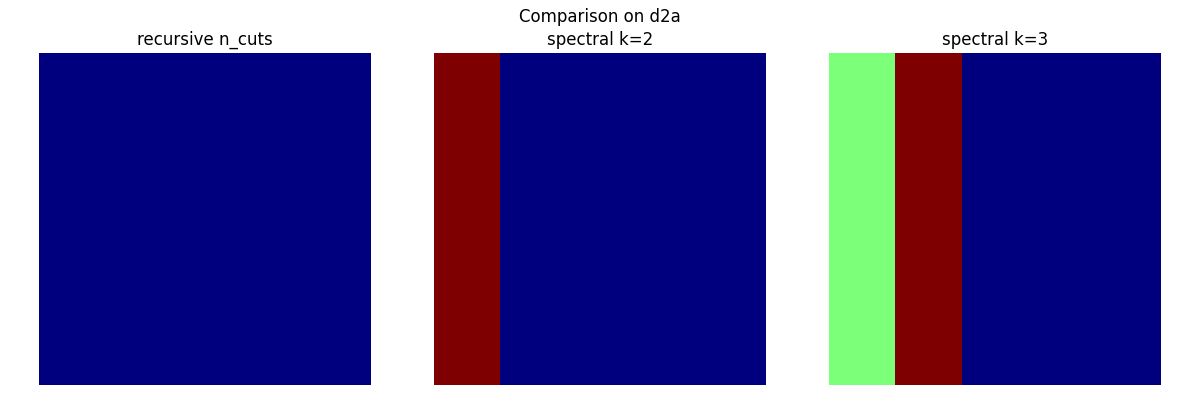
\includegraphics[width=0.9\textwidth]{d2a_comparison.png}
    \caption{Σύγκριση \en Recursive n-cuts \gr και \en Spectral Clustering \gr για την εικόνα \en \texttt{d2a}\gr}
\end{figure}

\begin{figure}[H]
    \centering
    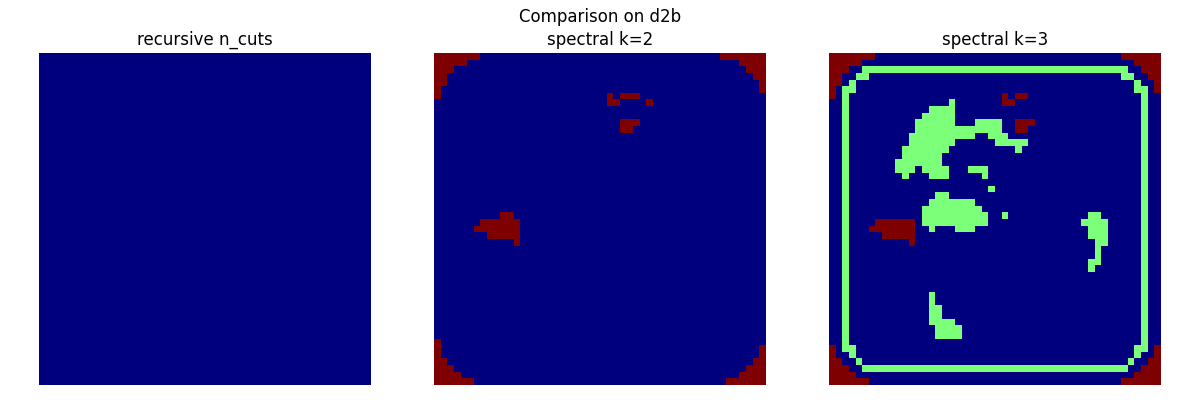
\includegraphics[width=0.9\textwidth]{d2b_comparison.png}
    \caption{Σύγκριση \en Recursive n-cuts \gr και \en Spectral Clustering \gr για την εικόνα \en \texttt{d2b}\gr}
\end{figure}

\vspace{0.3cm}
\noindent Τα πλήθη κόμβων σε κάθε \en cluster \gr που προέκυψαν είναι τα εξής:

\en
\begin{itemize}
    \item \texttt{d2a}, \textit{recursive}: \texttt{[2500]} \gr (δεν έγινε περαιτέρω διάσπαση λόγω υψηλής τιμής \en \texttt{Ncut}) \gr \en
    \item \texttt{d2a}, \textit{spectral k=2}: \texttt{[2000, 500]}
    \item \texttt{d2a}, \textit{spectral k=3}: \texttt{[1500, 500, 500]}

    \item \texttt{d2b}, \textit{recursive}: \texttt{[2500]} \gr (δεν έγινε περαιτέρω διάσπαση) \en
    \item \texttt{d2b}, \textit{spectral k=2}: \texttt{[2399, 101]}
    \item \texttt{d2b}, \textit{spectral k=3}: \texttt{[2062, 97, 341]}
\end{itemize}
\gr

\subsubsection{Σχολιασμός και Σύγκριση}

\textbf{Για την εικόνα \en d2a\gr}:
\begin{itemize}
    \item Η \en \texttt{recursive n-cuts} \gr επέστρεψε ένα μόνο \en cluster \gr (ολόκληρη η εικόνα ως μία ομάδα), γεγονός που φαίνεται αρχικά αντιφατικό με τα αναμενόμενα αποτελέσματα.
    \item Αυτό όμως εξηγείται πλήρως αν αναλυθεί η ροή της συνάρτησης \en \texttt{n\_cuts\_recursive()}\gr:
    \begin{itemize}
        \item Ο αρχικός διαχωρισμός του γράφου γίνεται μέσω \en \texttt{n\_cuts()}\gr με $k=2$.
        \item Στη συνέχεια υπολογίζεται η τιμή \en \texttt{Ncut} \gr του διαχωρισμού.
        \item Αν η τιμή \en \texttt{Ncut} \gr είναι μεγαλύτερη ή ίση από το κατώφλι \en \texttt{T2}\gr, η ομάδα δεν διασπάται περαιτέρω και καταχωρείται ως έχει.
    \end{itemize}
    \item Στην περίπτωση του \en \texttt{d2a}\gr, η αρχική τιμή \en \texttt{Ncut} \gr είναι αρκετά υψηλή (πάνω από 0.2), συνεπώς η διάσπαση απορρίφθηκε και το σύνολο των 2500 κόμβων παρέμεινε ως ένα ενιαίο \en cluster\gr.
    \item Αντιθέτως, η μέθοδος \en spectral clustering \gr δεν έχει κάποιο φραγμό ποιότητας, αλλά επιβάλλει αυστηρά την παραγωγή $k$ ομάδων — ανεξάρτητα από το αν αυτές έχουν ουσιαστική σημασία ή όχι.
    \item Για $k=3$ και $k=2$ στην εικόνα \en \texttt{d2a}\gr, οι ομάδες που προκύπτουν φαίνονται εύλογες και αποδίδουν καλύτερη διαχωριστική πληροφορία από την αναδρομική \en \texttt{n-cuts}\gr, για τις συγκεκριμένες παραμέτρους.
\end{itemize}

\hspace{-0.6cm}\textbf{Για την εικόνα \en d2b\gr}:
\begin{itemize}
    \item Αντίστοιχα με το \en \texttt{d2a}\gr, η \en \texttt{recursive n-cuts} \gr δεν προχώρησε σε περαιτέρω διαχωρισμό επειδή η αρχική τιμή \en \texttt{Ncut} \gr υπερέβη το κατώφλι \en \texttt{T2 = 0.2}\gr.
    \item Επομένως, η εικόνα θεωρήθηκε μη διασπάσιμη και επιστράφηκε ως ένα ενιαίο σύνολο 2500 κόμβων.
    \item Στην πράξη όμως, η εικόνα \en \texttt{d2b} \gr έχει μεγαλύτερη πολυπλοκότητα και κρύβει περισσότερες τοπικές δομές.
    \item Η \en \texttt{spectral clustering} \gr με $k=3$ καταφέρνει να εντοπίσει κάποιες από αυτές, αποδίδοντας διαφορετικές περιοχές, παρότι τα όρια μεταξύ τους δεν είναι τόσο καθαρά.
    \item Αυτό καταδεικνύει πως η \en \texttt{n\_cuts\_recursive} \gr είναι πολύ ευαίσθητη στην επιλογή του \en \texttt{T2}\gr. Αν είναι πολύ αυστηρό, τότε δεν γίνονται καν βασικές διασπάσεις.
\end{itemize}

\vspace{0.3cm}
\noindent \textbf{Συμπερασματικά:}
Η \en \texttt{n\_cuts\_recursive} \gr προσφέρει προσαρμοστικότητα και αποφυγή υπερδιάσπασης, αλλά εξαρτάται κρίσιμα από τη ρύθμιση του κατωφλιού \en \texttt{T2}\gr, που δρα ως φίλτρο ποιότητας. Αντίθετα, η \en \texttt{spectral clustering} \gr επιβάλλει $k$ ομάδες και αποδίδει πάντα αποτέλεσμα, ανεξαρτήτως ποιότητας. Στο συγκεκριμένο πείραμα, η \en \texttt{T2 = 0.2} \gr αποδείχθηκε υπερβολικά αυστηρή και δεν επέτρεψε την αποκάλυψη της υποκείμενης δομής, σε αντίθεση με τη \en \texttt{spectral clustering} \gr που εμφάνισε περισσότερα διαχωριστικά χαρακτηριστικά.

\subsubsection{Πείραμα με παραμετροποίηση \(\boldsymbol{T_1 = 1000}\), \(\boldsymbol{T_2 = \infty}\)}

\noindent Στο πείραμα αυτό, επιλέχθηκε υψηλή τιμή για το κατώφλι ελάχιστου μεγέθους ομάδας (\(T_1 = 1000\)) και απενεργοποιήθηκε ο έλεγχος της τιμής \en Ncut \gr (\(T_2 = \infty\)). Με αυτό τον τρόπο, η συνάρτηση \en \texttt{n\_cuts\_recursive} \gr αναγκάζεται να διαιρεί οποιαδήποτε ομάδα μεγαλύτερη των 1000 κόμβων, ανεξαρτήτως της ποιότητας του διαχωρισμού, με σκοπό να εξεταστεί η συμπεριφορά της μεθόδου υπό καθαρά δομικά κριτήρια μεγέθους.

\vspace{0.3cm}
\noindent \textbf{Αποτελέσματα Ομαδοποίησης:}
\en
\begin{itemize}
    \item \texttt{d2a}, \textit{recursive}: \texttt{[1000, 6, 11, 47, 8, 340, 87, 461, 540]} \gr (σύνολο 9 ομάδες) \en 
    \item \texttt{d2a}, \textit{spectral k=2}: \texttt{[2000, 500]}
    \item \texttt{d2a}, \textit{spectral k=3}: \texttt{[1500, 500, 500]}
    \item \texttt{d2b}, \textit{recursive}: \texttt{[359, 758, 382, 332, 669]} \gr (σύνολο 5 ομάδες) \en 
    \item \texttt{d2b}, \textit{spectral k=2}: \texttt{[2399, 101]}
    \item \texttt{d2b}, \textit{spectral k=3}: \texttt{[2062, 97, 341]}
\end{itemize}
\gr

\begin{figure}[H]
    \centering
    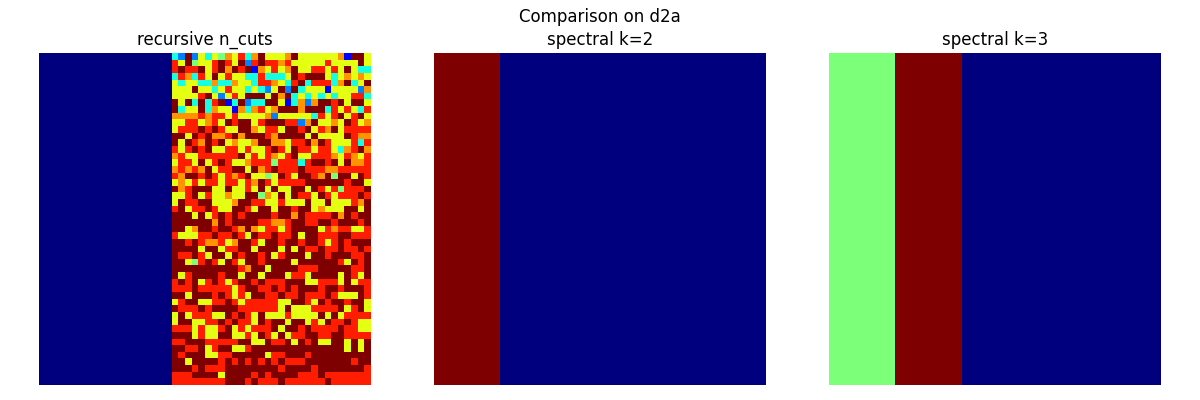
\includegraphics[width=0.9\textwidth]{d2a_comparison_tunedTs.png}
    \caption{Σύγκριση \en Recursive n-cuts \gr με \en Spectral Clustering \gr για την εικόνα \en \texttt{d2a} \gr με \(T_1 = 1000\), \(T_2 = \infty\)}
\end{figure}

\begin{figure}[H]
    \centering
    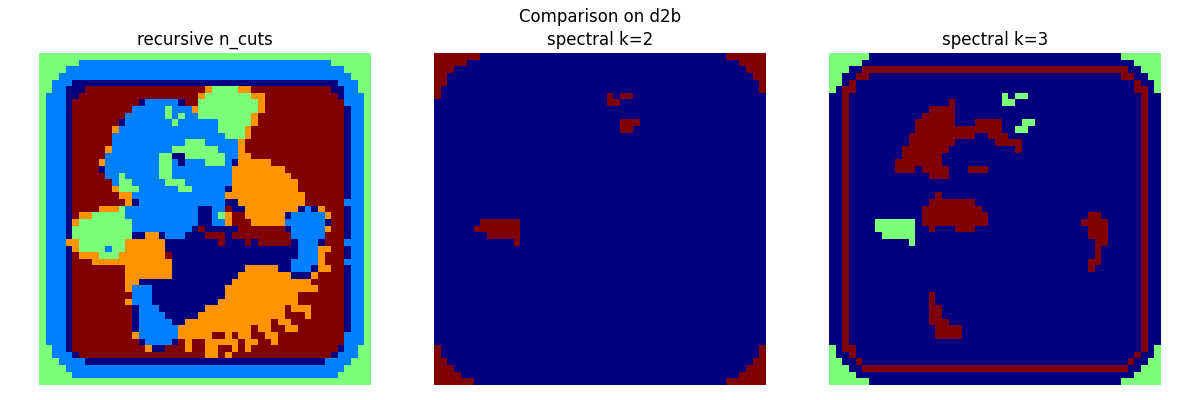
\includegraphics[width=0.9\textwidth]{d2b_comparison_tunedTs.png}
    \caption{Σύγκριση \en Recursive n-cuts \gr με \en Spectral Clustering \gr για την εικόνα \en \texttt{d2b} \gr με \(T_1 = 1000\), \(T_2 = \infty\)}
\end{figure}

\vspace{0.4cm}
\hspace{-0.6cm}\textbf{Σχολιασμός:}

\textbf{Για την εικόνα \en d2a\gr:}
\begin{itemize}
    \item Η μέθοδος \en \texttt{recursive n-cuts} \gr οδηγεί σε υπερδιάσπαση, όπως είναι αναμενόμενο λόγω του χαμηλού \(T_1\) και της απουσίας ελέγχου ποιότητας διαχωρισμού (αφού \(T_2 = \infty\)).
    \item Παρατηρείται έντονος θόρυβος στις μικρές περιοχές — δημιουργούνται πολύ μικρές ομάδες (π.χ. 6, 8, 11 κόμβοι) χωρίς ουσιαστικό νόημα.
    \item Η μέθοδος \en spectral clustering \gr, ιδιαίτερα για \(k=3\), καταφέρνει καλύτερα να διατηρήσει τη λογική χωρική κατανομή των περιοχών.
\end{itemize}

\textbf{Για την εικόνα \en d2b\gr:}
\begin{itemize}
    \item Η \en recursive n-cuts \gr παρουσιάζει μια πολύ πιο πλούσια και λεπτομερή τμηματοποίηση, αποκαλύπτοντας λειτουργικά ξεχωριστές περιοχές (π.χ. πρόσωπο, σώμα, καπέλο).
    \item Η \en spectral clustering \gr περιορίζεται σε μακροσκοπικά σχήματα (ιδιαίτερα για \(k=2\)) και αποτυγχάνει να εντοπίσει μικρότερες δομές.
\end{itemize}

\vspace{0.3cm}
\noindent \textbf{Συμπεράσματα:}
\begin{itemize}
    \item Η απενεργοποίηση του ελέγχου ποιότητας (\(T_2 = \infty\)) οδηγεί σε υπερκατάτμηση της εικόνας, ειδικά όταν επιβάλλεται μεγάλος αριθμός διαχωρισμών λόγω μικρού \(T_1\).
    \item Αν και αυτό είναι επιθυμητό σε σύνθετες εικόνες όπως η \en \texttt{d2b}\gr, καθώς αποδίδει περισσότερη λεπτομέρεια, είναι επιβλαβές για απλές περιπτώσεις όπως η \en \texttt{d2a}\gr.
    \item Το πείραμα αναδεικνύει τη σημασία της κατάλληλης ρύθμισης των παραμέτρων \en T1 \gr και \en T2 \gr για τον έλεγχο της λεπτομέρειας και της συνοχής της τμηματοποίησης.
\end{itemize}

\vspace{0.3cm}

\hspace{-0.6cm} Οι αντίστοιχοι κώδικες για αυτό το \en Chapter \gr βρίσκονται στα αρχεία \en \texttt{n\_cuts.py}, \texttt{demo3a.py}, \texttt{demo3b.py} \gr και \en \texttt{demo3c.py} \gr αντίστοιχα.


\bibliographystyle{plain}
\begin{thebibliography}{1}
    \bibitem{first_bibl}
    \en https://docs.scipy.org/doc/scipy/reference/generated/scipy.sparse.linalg.eigs.html
    \bibitem{second_bibl}
    \en https://elearning.auth.gr/course/view.php?id=16312
\end{thebibliography}

\end{document}